\documentclass[hidelinks, 12pt, oneside]{article}
\usepackage{bookmark}
\usepackage{graphicx}
\usepackage{hyperref}
\usepackage{titlesec}
\setcounter{secnumdepth}{4}
\usepackage[utf8]{inputenc}
\usepackage[english]{babel}
\usepackage{color}


\begin{document}

	\begin{center}
    \centering
    
%University logo
    
\includegraphics[width=144px]{img/icon.png}
    \rule{0\linewidth}{0.15\linewidth}\par
    
    		\begin{center}
		{\uppercase{\Large User Manual\par}}
   		{\Large iCrawler \par}
   			\vspace{1cm} 
   		{\Large Emilio Mumba  \par} 
    		\vspace{1cm}
		   		
    		{\Large The 5 Concurrent Nodes \par} 
    		\vspace{1cm}
		
		{\normalsize Khathutshelo Shaun Matidza\par}
		{\normalsize Sylvester Sandile Mpangane\par}
		{\normalsize Thabang Michael Letageng\par}
		{\normalsize Matthew Nel\par}
		
		\end{center}

		\textbf{}		
		\centering
		\vspace{2cm}
		Department of Computer Science, University of Pretoria

		
	 	{\Large  September 2015}
\end{center}
\clearpage


	\tableofcontents
	\newpage
	
	\section{Overview}
	\emph{iCrawler} is a monitoring app available for Android only. The app
	 uses your device's internet connection to send data logs collected from your phone to a desktop-dashboard
	 for review. The app is absolutely free to download.\newline\newline
	 
	 \uppercase{Why use iCrawler:}\newline
	 \begin{itemize}
		\item Child monitoring\newline
		\emph{iCrawler} can be use by parents/guardians to monitor activities that their minor
		 children get up to.	
		\item Employee monitoring\newline
		Companies that give their employees mobile devices can use the \emph{iCrawler} to monitor any 
		unauthorized activities that employees may get up to.
	\end{itemize}
	\newpage
	
	
	\section{Configuration}
	iCrawler operates on mobile devices running on android operating system. It is compatible with Android 4.2 API level 11 and higher versions. The application runs on start up in the background once installed and requires internet connection in order to allow a user to register a device and save data onto a database. Data saved in a database can be viewed using any major Internet browser. After installation on the device, to use iCrawler you will need to register and login. \
	
	\section{Installation}\newpage
	
	\section{Getting Started}
	After successful installation, locate the iCrawler app icon and click on it to run the app.\
	
	 \begin{itemize}
	 	\item \textbf{Terms and Conditions}\newline
	 	Before you can use iCrawler you neeed to read the 'Terms and Conditions' on startup and only 
	 	after accepting them can you proceed, if you don't accept you can not use the app.
	 	 
	 	 %terms and conditions screenshot here%
	 	 \begin{figure}[h!]
	 	 	\caption{Terms and Conditions page}
	 	 	\centering 																												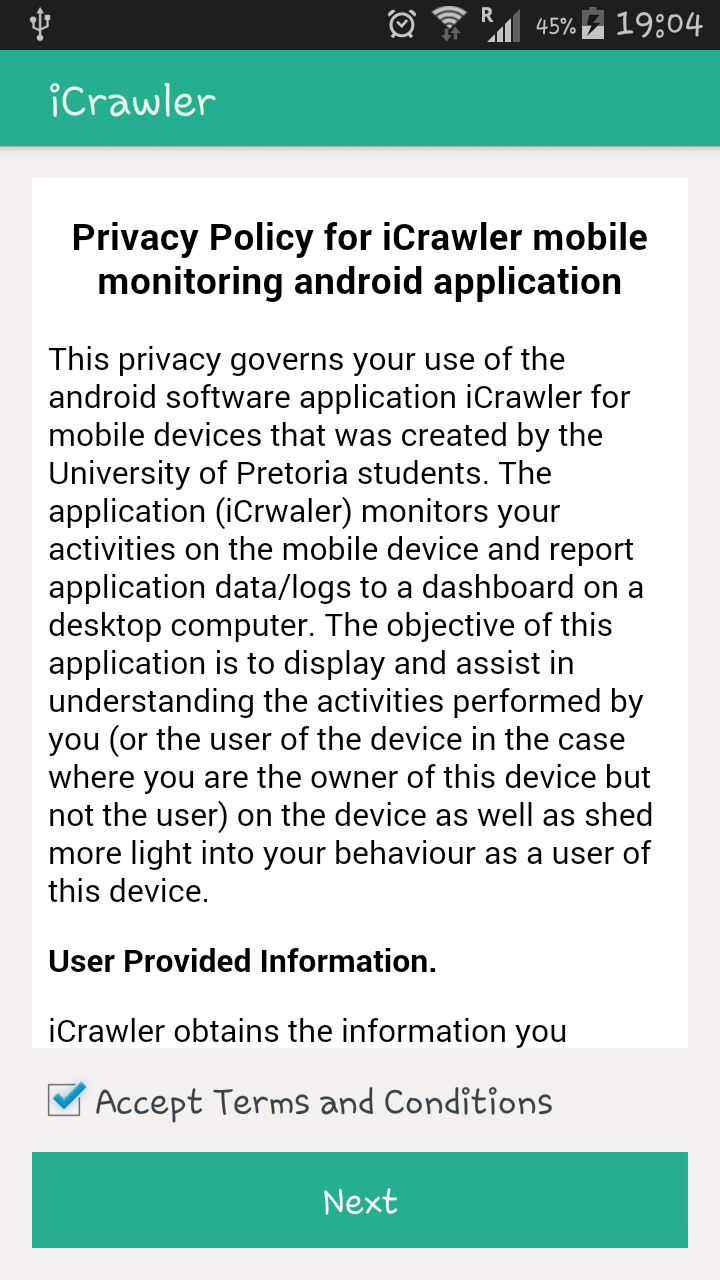
\includegraphics[width=0.5 \textwidth]{img/tnc2.png}
	 	 \end{figure}\newpage
	 	 
	 	\item \textbf{Sign up new user}\newline
	 	If you are a first time user you need to sign up after accepting the 'Terms and Conditions'. You need
	 	to provide a working \emph{email address} and create a \emph{password} you will use to sign in with in future.
	 	If you have an existing account, simply 'click Sign in' to go to the sign in page.
	 	 
	 	 %register new user screenshot here%
	 	 \begin{figure}[h!]
	 	 	\caption{Sign up user page}
	 	 	\centering 																												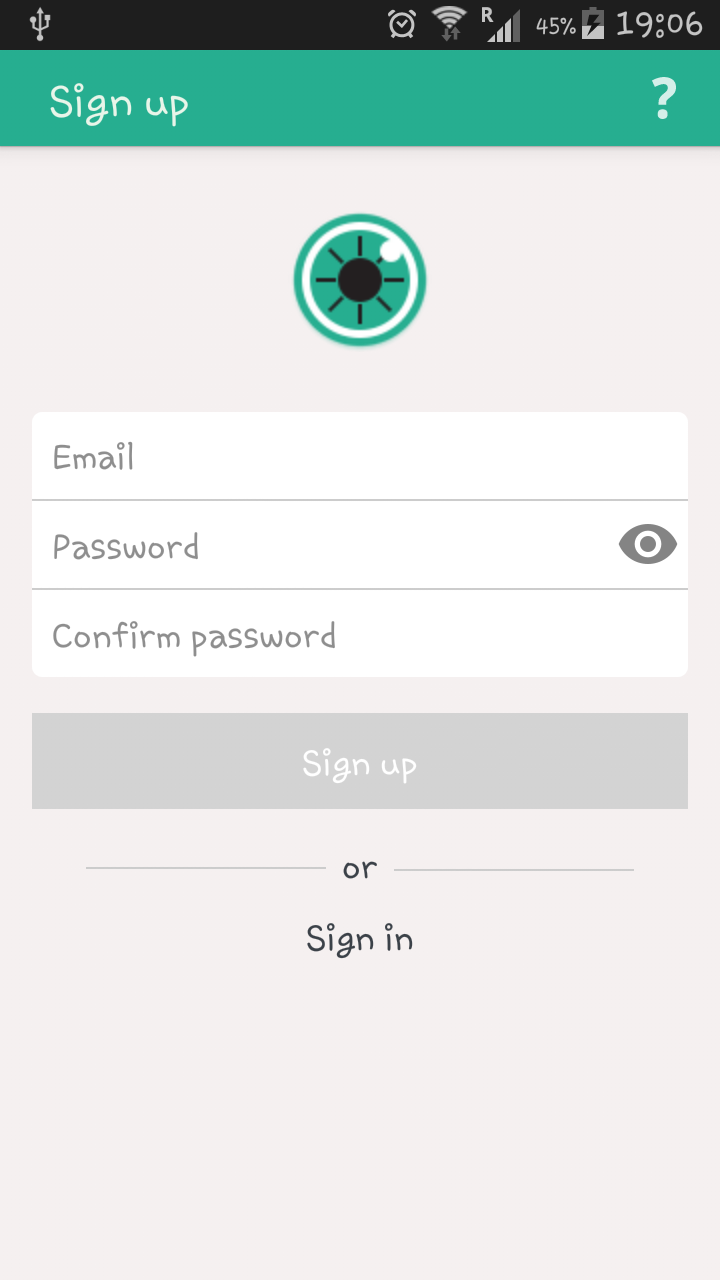
\includegraphics[width=0.5 \textwidth]{img/reg.png}
	 	 \end{figure}\newpage
	 	 
	 	\item \textbf{Sign in as existing user}\newline
	 	If you have used the iCrawler app before, you need not to sign up again, simply enter your credentials and then
	 	'click Sign in' in order to subscribe the new device. If not, 'click Sign up' to register as a new user.
	 	
	 	%login user screenshot here%
	 	 \begin{figure}[h!]
	 	 	\caption{Sign in user page}
	 	 	\centering 																												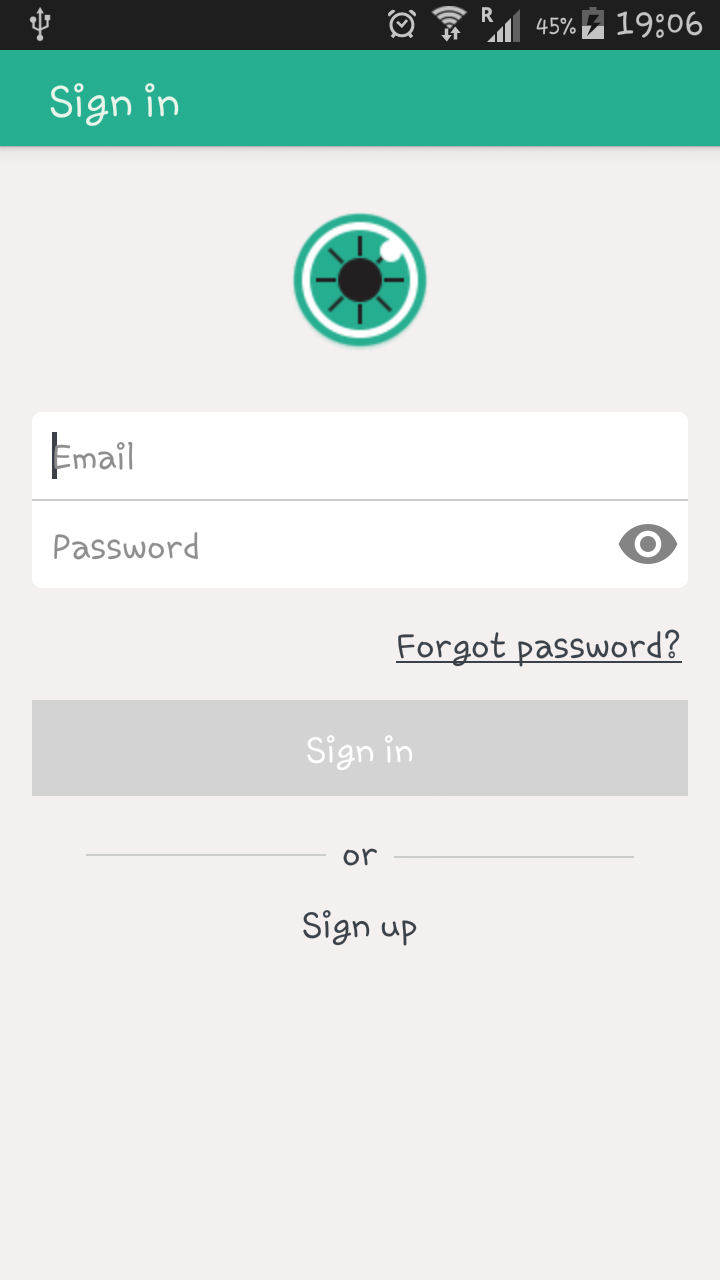
\includegraphics[width=0.5 \textwidth]{img/log.png}
	 	 \end{figure}
	 	 
	 \end{itemize}\newpage
	 
	 
	\section{Using the App}
	The app runs in the background after 'Signing up or Signing in'; there is no other form of interaction with 
	the app thereafter. You can access the log reports generated via the dashboard.
	\newline\newline
	
	\section{Troubleshooting}
	The following section lists some common issues and their resolutions.
	\textbf{iCrawler does not launch.}
	Restart your phone and try to launch the application again.
	\textbf{iCrawler crashes immediately after launch.}
	Ensure that your device meets the minimum specifications to run iCrawler (See configurations).
	Go to Settings -> Apps -> Manage Apps ->Running, to check if your apps are not using up all your memory. Try to end all processes you do not need and re-start your phone.
	\textbf{Other unknown causes.}
	 If problems continue, delete the app completely and then reinstall it from Google Play. And if this does not solve the issue, contact our support: support@iCrawler.co.za\
			
\end{document}
